\section{Experimental Evaluation}
\label{sec:exp}

We now describe in detail our experimental analysis. For additional information, we make all our material publicly available online~\cite{ourcode} and provide an interactive WebApp~\cite{ourwebsite} for navigating and exploring the experimental results.

\journalv{The experimental section is organized as follows:
\begin{itemize}%[noitemsep,topsep=0pt,parsep=0pt,partopsep=0pt,leftmargin=0.5cm]
    \item In \textbf{Section~\ref{exp:setup}}, we first start by introducing the datasets and the methods to evaluate the previously defined model selection baselines. We also define the performance measures.
    \item In \textbf{Section~\ref{exp:overalleval}}, we then conduct an extensive evaluation of both accuracy (classification and anomaly detection) and execution time for all model selection methods and over the entire benchmark.
    \item In \textbf{Section~\ref{exp:windowlength}}, we analyze more precisely the influence of the window length of our proposed pipeline.
    \item In \textbf{Section~\ref{exp:datasets}}, we measure the influence of datasets and anomalies characteristics on the performances of the model selection algorithms.
    \item In \textbf{Section~\ref{exp:detectionvsclass}}, we measure the correlation between classification accuracy (i.e., of the model selection methods) and anomaly detection accuracy. We proposed empirical lower and upper bounds that contain the minimal and the maximal performances of any model selection algorithms for a given classification accuracy.
    \item In \textbf{Section~\ref{exp:sup2unsup}}, we finally measure the accuracy of model selection methods when used in an unsupervised manner (i.e., used for time series from domains that were not included in the training set). 
\end{itemize}}

\journalv{\subsection{Experimental Setup and Settings}}
\label{exp:setup}

\begin{table*}[tb]
    \centering
    \caption{\journalv{Summary of datasets, methods, and measures used in this experimental evaluation.}}
        \scalebox{0.8}{
        \begin{tabular}{|c|c|}
        \hline
        \rowcolor{Gray}
        \textbf{Datasets} & \textbf{Description} \\
        \hline
        Dodgers~\cite{10.1145/1150402.1150428} & unusual traffic after a Dodgers game \textbf{(1 time series)}\\ 
        \hline
        ECG~\cite{Moody} & standard electrocardiogram dataset \textbf{(52 time series)}\\ 
        \hline
        IOPS~\cite{IOPS} & performance indicators of a machine \textbf{(58 time series)}\\ 
        \hline
        KDD21~\cite{kdd21} & composite dataset released in a recent SIGKDD 2021 \textbf{(250 time series)}\\ 
        \hline
        MGAB~\cite{markus_thill_2020_3762385} & Mackey-Glass time series with non-trivial anomalies \textbf{(10 time series)}\\ 
        \hline
        NAB~\cite{ahmad_unsupervised_2017} &  Web-related real-world and artificial time series \textbf{(58 time series)}\\ 
        \hline
        SensorScope~\cite{YAO20101059} & environmental data \textbf{(23 time series)}\\ 
        \hline
        YAHOO~\cite{yahoo} & \makecell{ time series based on Yahoo production systems \textbf{(367 time series)}}\\ 
        \hline
        Daphnet~\cite{5325884} & acceleration sensors on Parkinson's disease patients \textbf{(45 time series)}\\ 
        \hline
        GHL~\cite{filonov2016multivariate} & Gasoil Heating Loop telemetry \textbf{(126 time series)}\\ 
        \hline
        Genesis~\cite{vonBirgelen2018} & portable pick-and-place demonstrator \textbf{(6 time series)}\\ 
        \hline
        MITDB~\cite{Moody} & ambulatory ECG recordings \textbf{(32 time series)}\\ 
        \hline
        OPPORTUNITY~\cite{5573462} & motion sensors for human activity recognition \textbf{(465 time series)}\\ 
        \hline
        Occupancy~\cite{CANDANEDO201628} & temperature, humidity, light, and CO2 of a room \textbf{(10 time series)}\\ 
        \hline
        SMD~\cite{10.1145/3292500.3330672} & Server Machine telemetry \textbf{(281 time series)}\\ 
        \hline
        SVDB~\cite{greenwald_improved_1990} & ECG recordings \textbf{(115 time series)}\\ 
        \hline
        \hline
        \rowcolor{Gray}
        \textbf{Anomaly Detection} & \textbf{Description} \\
        \hline
        IForest~\cite{liu_isolation_2008} & \makecell{constructs binary trees based on random space splitting. The nodes (i.e., \\ subsequences) with shorter paths to the root are more likely to be anomalies. }\\
        \hline
        IForest1~\cite{liu_isolation_2008}  & same as IForest, but each point (individually) are used as input. \\
        \hline
        LOF~\cite{Breunig:2000:LID:342009.335388} & computes the ratio of the neighboring density to the local density.\\ 
        \hline
        MP~\cite{yeh_time_2018} & \makecell{detects abnormal subsequences with the largest nearest neighbor distance.} \\ 
        \hline
        NormA~\cite{boniol_unsupervised_2021} & \makecell{identifies normal patterns using clustering and calculates each subsequence \\ weighted distance (with statistical criteria) to the normal patterns.} \\ 
        \hline
        PCA~\cite{aggarwal_outlier_2017} & \makecell{projects data to a lower-dimensional hyperplane, and data points \\ with a significant distance from this plane can be identified as outliers.} \\ 
        \hline
        AE~\cite{10.1145/2689746.2689747} & \makecell{projects data to the lower-dimensional latent space and reconstructs the \\ data, and outliers are expected to have larger reconstruction errors.} \\ 
        \hline
        LSTM-AD~\cite{malhotra_long_2015} & \makecell{use an LSTM network that from the current subsequence tries to predict the \\ following value. The error prediction is then used to identify anomalies.}\\ 
        \hline
        POLY~\cite{li_unifying_2007} & \makecell{fits a polynomial model that tries to predict the time series values from the \\ previous subsequences. Outliers are detected with prediction error} \\ 
        \hline
        CNN~\cite{8581424} & \makecell{builds, using a convolutional neural network, a correlation between current \\ and previous subsequences. The anomaly score is the prediction deviation.} \\ 
        \hline
        OCSVM~\cite{scholkopf_support_1999} & \makecell{is a support vector method that fits the normal training dataset and finds the normal data's boundary.}\\ 
        \hline
        HBOS~\cite{goldstein2012histogram} & \makecell{builds a histogram for the time series. The anomaly score is the  inverse of the height of the bin.} \\
        \hline
        \hline
        \rowcolor{Gray}
        \textbf{Model Selection} & \textbf{Description} \\
        \hline
            % \rowcolor{lGray}
            % \multicolumn{2}{|c|}{\it Feature-based classifier} \\
            % \hline \trianbox1{featurebased}
        \cellcolor{featurebased} SVC~\cite{10.1145/130385.130401} &  \makecell{maps instances to points in space to maximize the gap between classes.}\\
        \hline
        \cellcolor{featurebased} Bayes~\cite{Zhang2004TheOO} & \makecell{uses Bayes' theorem to classify a point using each class posterior probabilities.} \\
        \hline
        \cellcolor{featurebased} MLP~\cite{Hinton1989ConnectionistLP} & \makecell{consists of multiple layers of interconnected neurons} \\
        \hline
        \cellcolor{featurebased} QDA~\cite{Geisser1964PosteriorOF} & is a discriminant analysis algorithm for classification problems \\
        \hline
        \cellcolor{featurebased} AdaBoost~\cite{10.5555/646943.712093} & \makecell{is a meta-algorithm using boosting technique with weak classifiers} \\
        \hline
        \cellcolor{featurebased} Decision Tree~\cite{Hunt1966ExperimentsII} & \makecell{is an approach that splits data points into separate leaves based on features} \\
        \hline
        \cellcolor{featurebased} Random Forest~\cite{598994} & \makecell{is a set of Decision Trees fed with random samples and features.} \\
        \hline
        \cellcolor{featurebased} kNN~\cite{Fix1989DiscriminatoryA} & \makecell{assigns the most common class among its k nearest neighbors.} \\
            % \hline
            % \rowcolor{lGray}
            % \multicolumn{2}{|c|}{\it Time series classifier} \\
        \hline
        \cellcolor{rocket} Rocket~\cite{dempster2021minirocket} & \makecell{transforms time series using a set of convolutional kernels, creating features used to train a linear classifier} \\
        \hline
            % \rowcolor{lGray}
            % \multicolumn{2}{|c|}{\it Convolutional-based neural networks}  \\
            % \hline
        \cellcolor{convbased} ConvNet~\cite{DBLP:journals/corr/WangYO16} & \makecell{uses convolutional layers to learn spatial features from the input data.} \\
        \hline
        \cellcolor{convbased} ResNet~\cite{DBLP:journals/corr/WangYO16} & \makecell{is a ConvNet with residual connections between convolutional block} \\
        \hline
        \cellcolor{convbased} Inception Time~\cite{fawaz2020inceptiontime} & \makecell{is a combination of ResNets with kernels of multiple sizes} \\
        \hline
            % \rowcolor{lGray}
            % \multicolumn{2}{|c|}{\it Transformer-based neural networks}  \\
            % \hline
        \cellcolor{transbased} SiT-conv~\cite{dosovitskiy2020image} & \makecell{is a transformer architecture with a convolutional layer as input} \\
        \hline
        \cellcolor{transbased} SiT-linear~\cite{dosovitskiy2020image} & \makecell{is a transformer architecture for which time series are divided into \\ non-overlapping patches and linearly projected into the embedding space} \\
        \hline
        \cellcolor{transbased} SiT-stem~\cite{xiao2021early} & \makecell{is a transformer architecture with convolutional layers with increasing dimensionality as input} \\
        \hline
        \cellcolor{transbased} SiT-stem-ReLU~\cite{wang2022scaled} & \makecell{is similar to SiT-stem but with Scaled ReLU.} \\
        \hline
        \hline
        \rowcolor{Gray}
        \textbf{\journalv{Evaluation}} & \textbf{\journalv{Description}} \\
        \hline
        Classification Accuracy &  \makecell{the number of correctly selected methods divided by the total number of time series}\\
        \hline
        % \rowcolor{lGray}
        % \multicolumn{2}{|c|}{\it Anomaly detection accuracy measures}  \\
        % \hline
        AUC-PR~\cite{10.1145/1143844.1143874} &  Area under the Precision-Recall curve\\
        \hline
        VUS-PR~\cite{10.14778/3551793.3551830} &  \makecell{Volume under the Precision-Recall surface (obtained from different length of a buffer region surrounding the anomalies)}\\
        \hline
        % \rowcolor{lGray}
        % \multicolumn{2}{|c|}{\it Execution Time measures}  \\
        % \hline
        Training Time & \makecell{number of seconds required to train a model selection method.} \\
        \hline
        Selection Time & \makecell{number of seconds required to predict the best model to use.} \\
        \hline
        Detection Time & \makecell{number of seconds required to compute an anomaly score. For model selection methods, \\it includes both the prediction of the model to use and the execution of the chosen model.} \\
        \hline
        \end{tabular}
        } 
        \label{SymbolTable}
\end{table*}

\noindent \textbf{Technical setup: }
We implemented the deep learning-based model selection methods in Python 3.5 using the PyTorch library~\cite{NEURIPS2019_bdbca288}. For the feature-based approach, we used the TSFresh~\cite{CHRIST201872} and scikit-learn~\cite{JMLR:v12:pedregosa11a} libraries. We then used sktime~\cite{Lning2019sktimeAU} for the Rocket algorithm implementation. For the anomaly detection methods, we used the implementation provided in the TSB-UAD benchmark~\cite{10.14778/3529337.3529354}. The evaluation was conducted on a server with Intel Core i7-8750H CPU 2.20GHz x 12, with 31.3GB RAM, and Quadro P1000/\journalv{PCIe}/SSE2 GPU with 4.2GB RAM, and on Jean Zay cluster with Nvidia Tesla V100 SXM2 GPU with 32 GB RAM.

\noindent \textbf{Datasets: }
For our evaluation purposes, we use the public datasets identified in the TSB-UAD benchmark~\cite{10.14778/3529337.3529354}. The latter corresponds to datasets (described in Table~\ref{SymbolTable}) proposed in the literature containing multiple time series with labeled anomalies. Specifically, each point in every time series is labeled as normal or abnormal.

\noindent \textbf{Anomaly Detection Methods: }
For the experimental evaluation, we select 12 different anomaly detection methods, summarized in Table~\ref{SymbolTable}. Out of these, 8 are fully unsupervised (i.e., they require no prior information on the anomalies to be detected): IForest, IForest1, LOF, MP, NormA, PCA, HBOS, and POLY. The remaining 4 methods are semi-supervised (i.e., they require some information related to normal behaviors), namely, OCSVM, AE, LSTM-AD, and CNN. For all these anomaly detection baselines, we set the parameter as described in the TSB-UAD benchmark~\cite{10.14778/3529337.3529354}.

\noindent \textbf{Method Selection baselines: }
We then consider the method selection baseline described in Section~\ref{sec:proposed} and summarized in Table~\ref{SymbolTable}. We first consider {\it feature-based} methods, that extract features using TSFresh~\cite{CHRIST201872} library to select the correct anomaly detection method. We then consider \journalv{Rocket}, state-of-the-art {\it time series classifier}. We also include two types of deep learning classifiers; (i) {\it Convolutional-based neural networks} and (ii) {\it Transformer-based neural networks}. Table~\ref{SymbolTable} summarizes the different model selection methods (i.e., classifiers). In total, we consider 16 methods, trained with window lengths $\ell$ equal to 16, 32, 64, 128, 256, 512, 768, and 1024. In total, we trained 128 models. In the following section, we refer to a model $M$ trained using a window length $\ell$ as $M$-$\ell$.

\noindent \textbf{Parameter settings: }
We use the same 70/30 split of the benchmark for all the classification models. Therefore, we can compare models trained on the same training set and evaluated on the same set of time series. Then, for the feature-based methods, we set the hyperparameters of the models based on the default parameters of scikit-learn. Moreover, for \journalv{Rocket}, we use 10000 kernels to extract the features and the logistic regression with stochastic gradient descent (computed in batches) for the classification step. Finally, for Convolutional and Transformer-based methods, we use a learning rate of $10^{-5}$, with a batch size of 256 and an early stopping strategy with a maximum of 50 epochs without improvement. Moreover, we use the weighted cross-entropy loss and set the maximum number of epochs to 10,000 (with a training time limit of 20 hours).

\noindent \textbf{Evaluation measures: }
We finally use four evaluation measures\journalv{, summarized in Table~\ref{SymbolTable}}. For model selection accuracy, we use the classification accuracy (i.e., the number of anomaly detectors correctly selected divided by the total number of time series). For anomaly detection accuracy, we use both AUC-PR~\cite{10.1145/1143844.1143874} and VUS-PR~\cite{10.14778/3551793.3551830} (with a buffer length equal to 10 points). For execution time, we measure the {\it training time} (i.e., the time required to train a model selection algorithm), the {\it selection time} (i.e., the time a model selection approach needs to predict which detector to use), and the {\it detection time} (i.e., the time required to predict which detector to use, and to execute it).

\begin{figure}
    \centering
    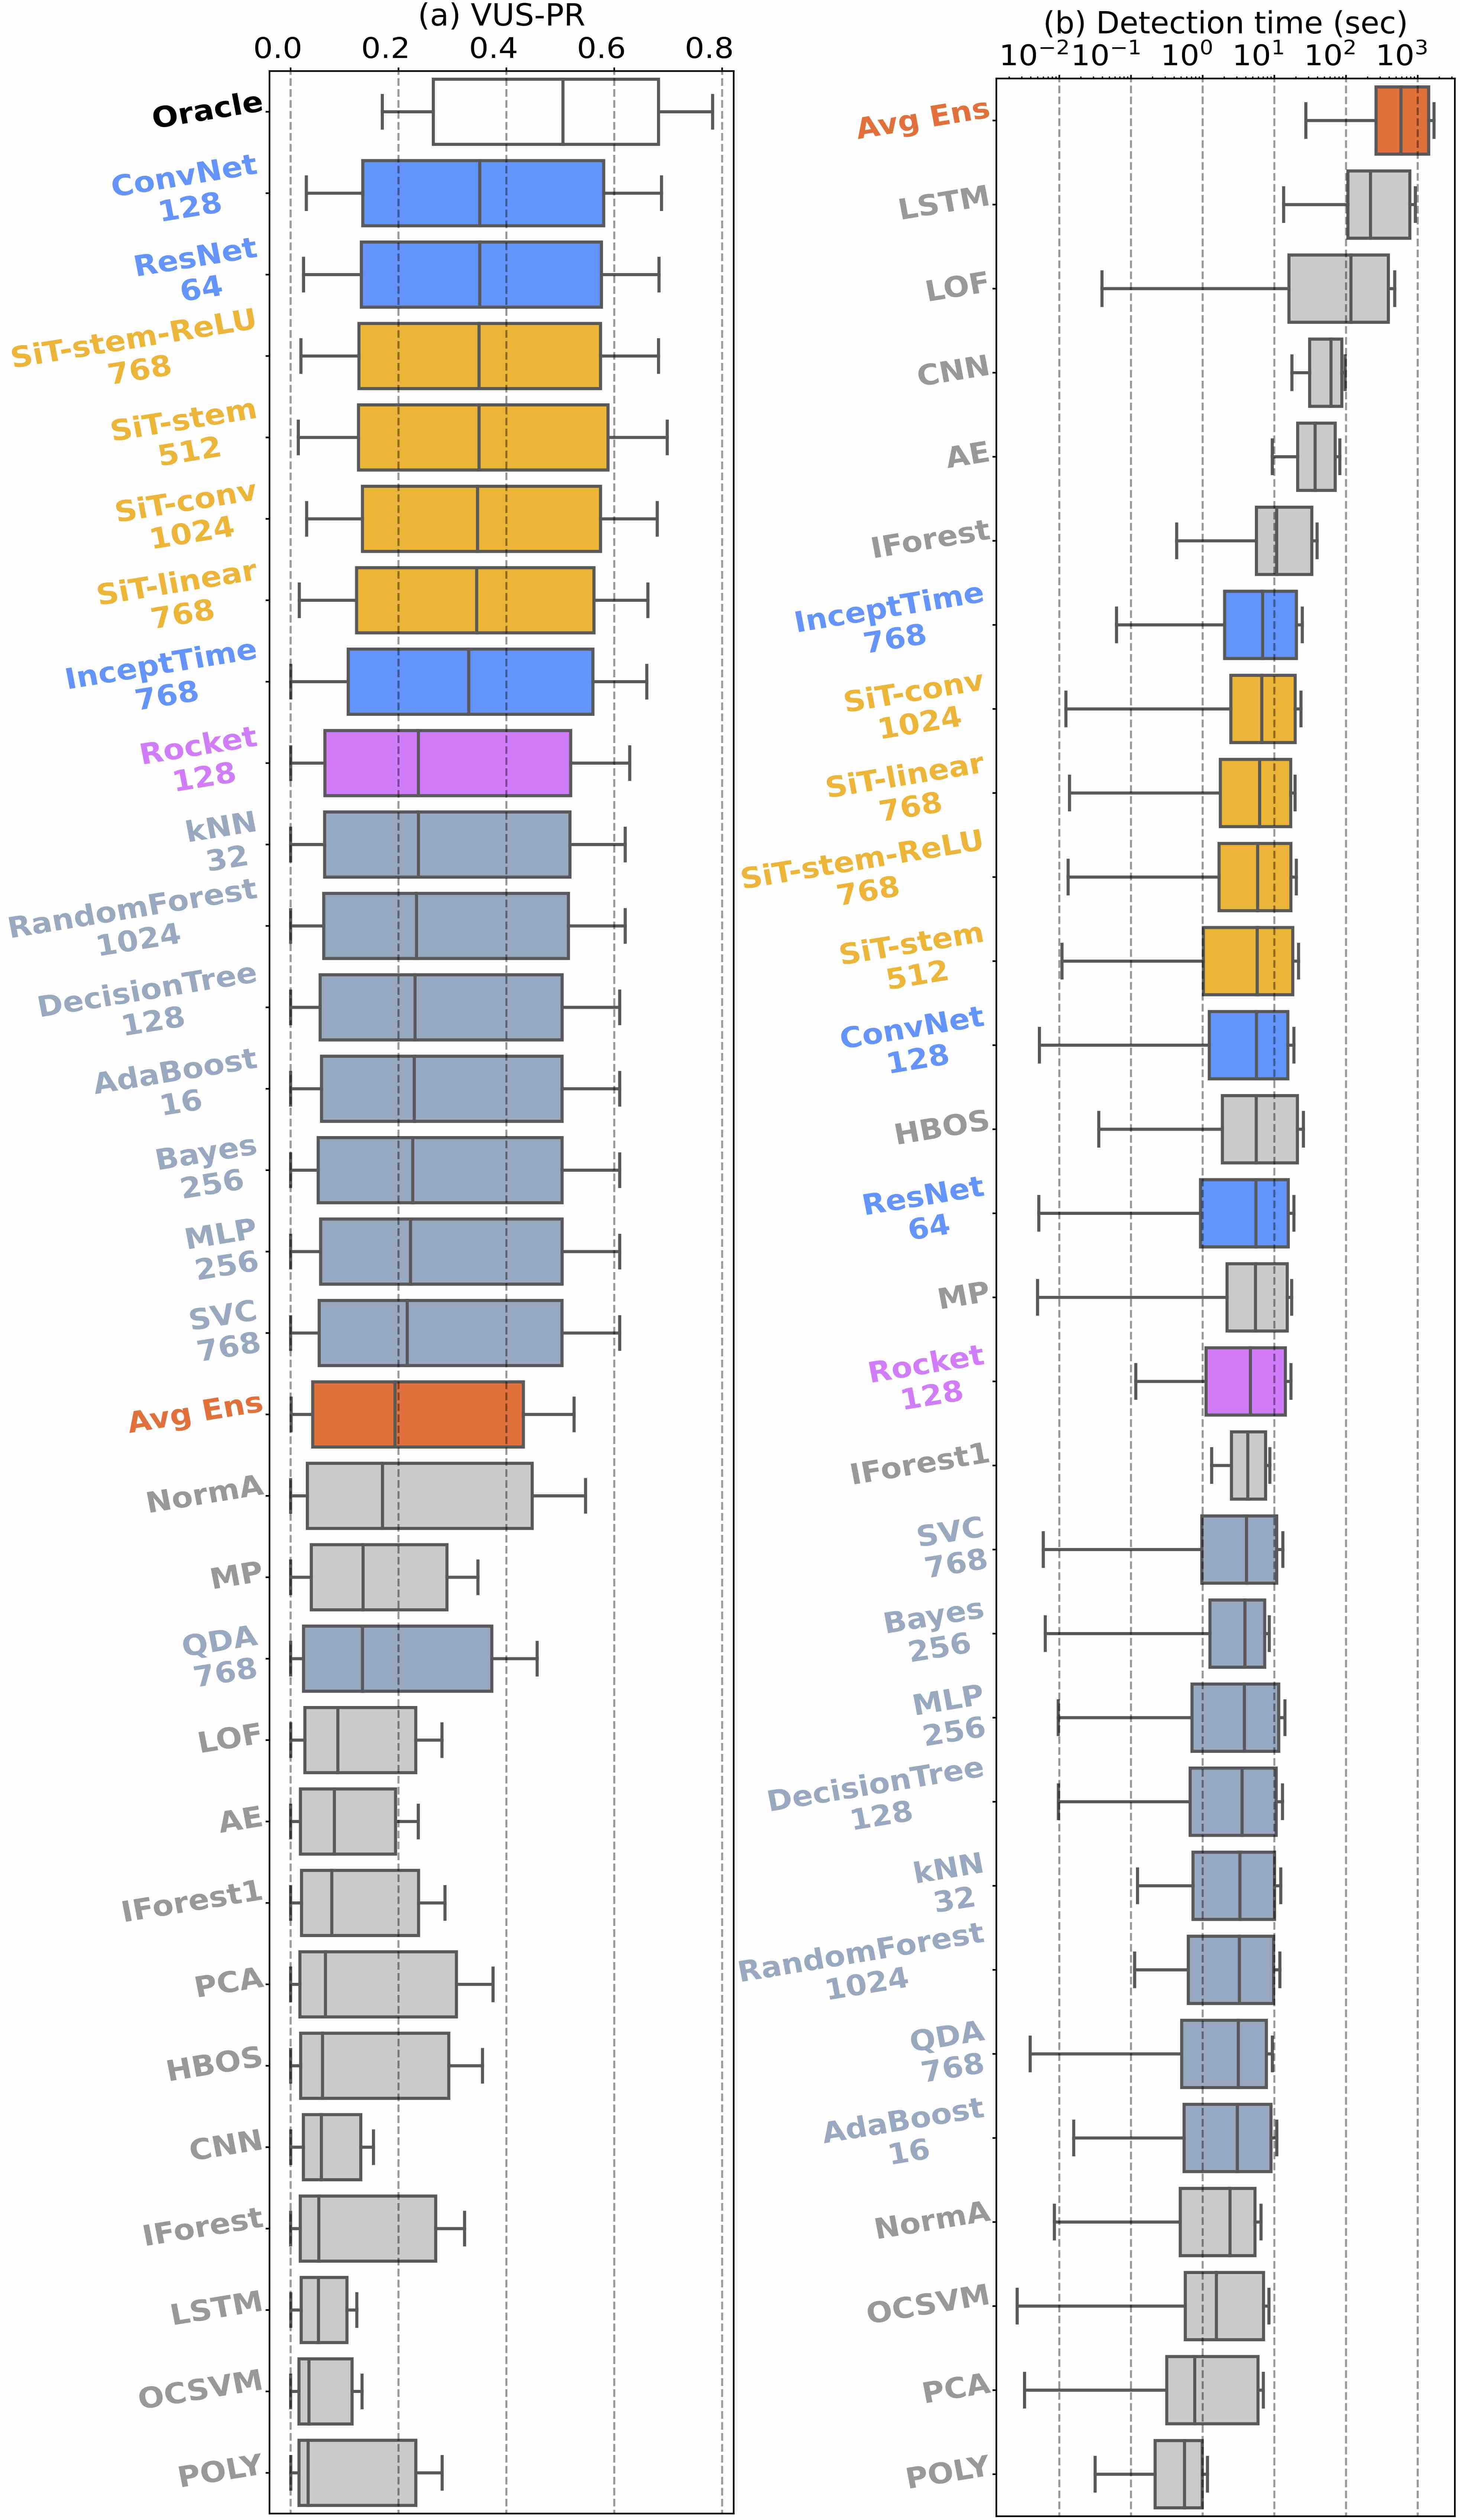
\includegraphics[width=1\linewidth]{figures/Fig5.jpg}
        \caption{VUS-PR and Detection time (seconds) for all model selection approaches (showing only the window length that maximizes VUS-PR for each model) over a test set of 497 series from TSB-UAD. \journalv{The methods are sorted: the most accurate methods are at the top (a); the fastest methods are at the bottom (b)}}
        \label{fig:overall_res}
\end{figure}


\subsection{Overall Evaluation}
\label{exp:overalleval}

We first evaluate accuracy (classification and anomaly detection) and execution time for all model selection methods over the entire benchmark. We split the benchmark into a train and test set with $1404$ and $496$ time series, respectively. Both sets contain time series from all datasets. Thus, the models have examples of all available domains. In Section~\ref{exp:sup2unsup}, we evaluate the performance of the models when applied to unseen (i.e., not used in the training set) datasets.

\subsubsection{\textbf{Accuracy Evaluation}}

We first analyze the accuracy of all model selection methods (using all window lengths) and compare them to the Oracle \journalv{(i.e. the perfect classifier),} the Averaging Ensemble method (Avg Ensemble) \journalv{(i.e., running all anomaly detection methods and returning the average of all anomaly scores),} and \journalv{the} anomaly detection methods in the TSB-UAD benchmark.

\begin{figure}
    \centering
    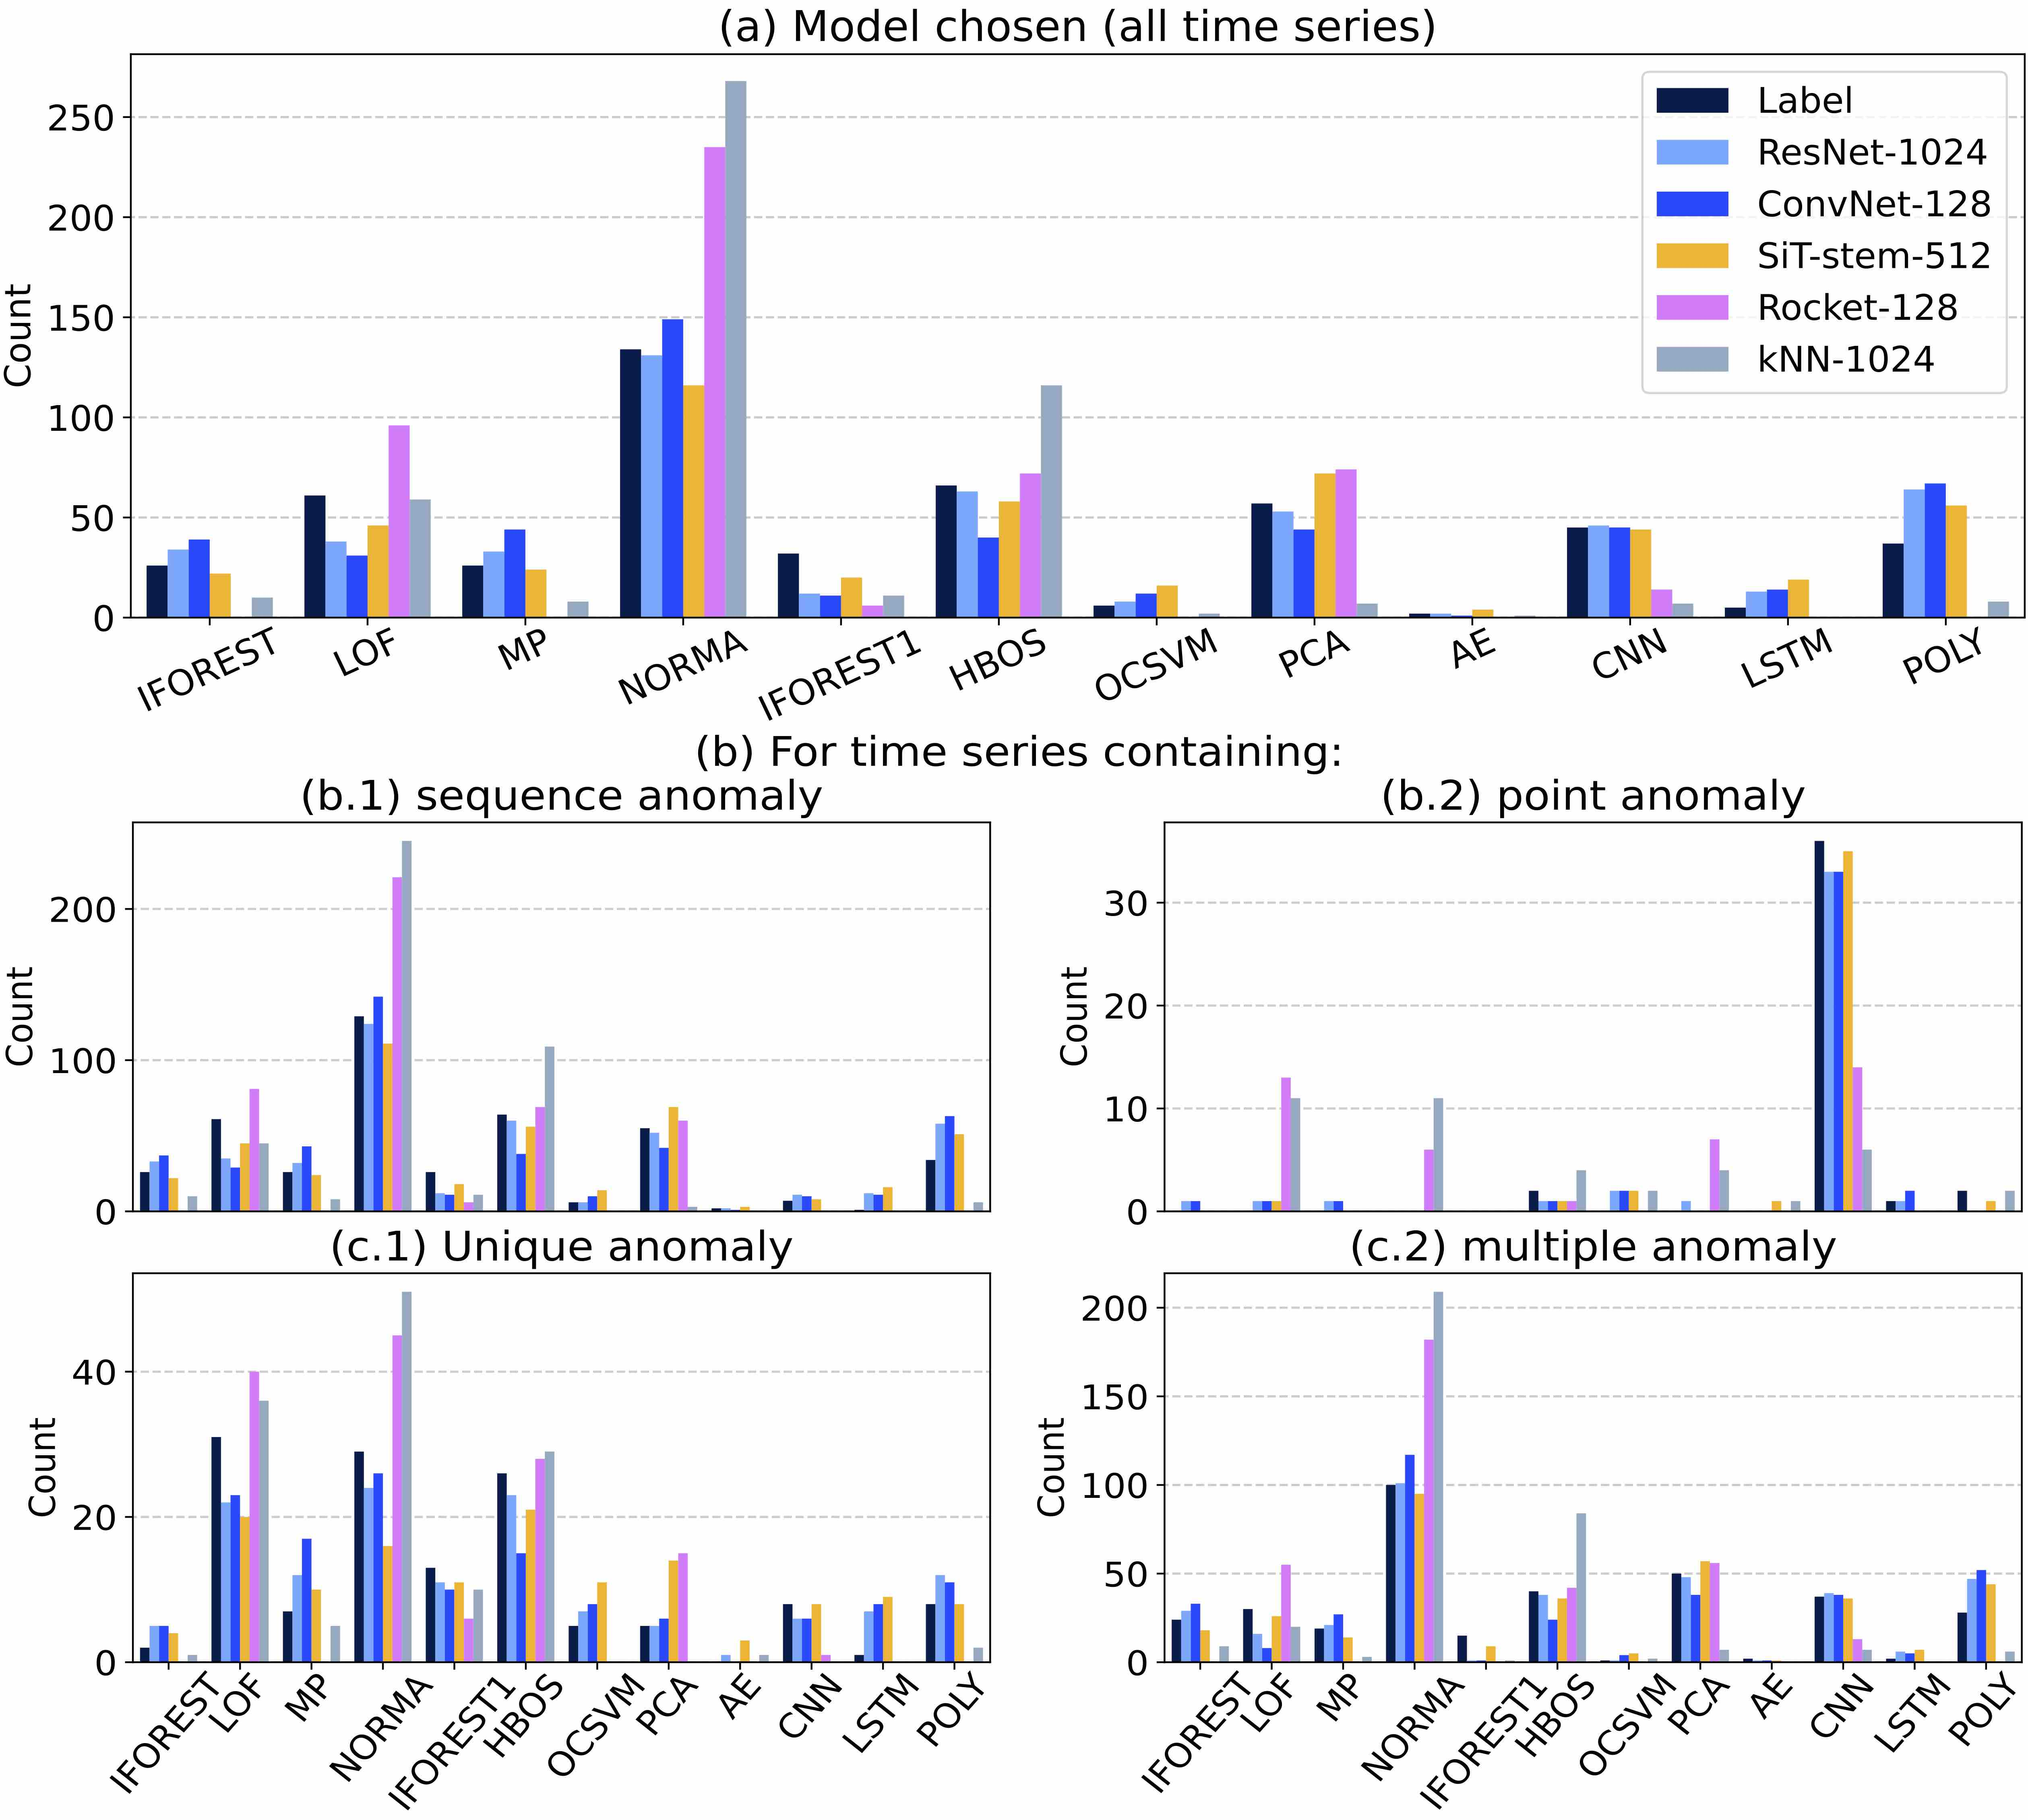
\includegraphics[width=\linewidth]{figures/Fig6.jpg}
        \caption{Distribution of the selected models for five models (the best for each category) compared to the distribution of the labels (in black). Difference of distributions between time series containing (b) sequence and point anomalies, and (c) unique or multiple anomalies.}
        \label{fig:classif_distrib}
\end{figure}

Figure~\ref{fig:overall_res} (a) depicts the overall VUS-PR over the entire TSB-UAD benchmark (i.e., each box-plot corresponds to 497 accuracy values for the 497 time series into the test set). The Convolutional-based approaches are in dark blue, the Transformer-based approaches are in yellow, the Feature-based approaches are in light blue, Rocket models are in violet, and the anomaly detection methods of the TSB-UAD benchmark are in light grey. The oracle is the top box plot (in white), and the Avg Ensemble is the orange box plot. The box-plot are sorted based on the median value. In total, we compare 142 models on 497 time series. In Figure~\ref{fig:overall_res}, we depict only the models with the window length that leads to the best VUS-PR.

First, almost all model selection methods outperform the existing anomaly detection methods. We also see that most model selection methods outperform the Avg Ensemble approach. Thus, we can conclude that model selection using time series classifiers significantly improves the state-of-the-art methods. 

More interestingly, we observe a partition in the ranking of the methods. First, Convolutional and Transformer-based approaches produce equivalent accuracy values and represent the top-48 methods. However, whereas all the Convolutional-based methods are in the top-48, a few of the Transformer-based approaches are further away in the ranking. Moreover, the first non-deep learning method is $rocket$-$128$ (ranked 49), followed closely by $knn$ models. We also observe that the $rocket$ approaches are very spread across the ranking ($rocket$-$128$ is ranked 50, and $rocket$-$16$ is ranked 124). This implies that the choice of window length strongly impacts accuracy. Overall, the best selection model is 2.8 times more accurate than the best anomaly detection method in TSB-UAD.

Then, we also note that all the model selection methods are significantly less accurate than the Oracle. For example, in Figure~\ref{fig:overall_res} (a), there is a gap of 0.2 VUS-PR between the Oracle and the best model selection method. Such a significant gap indicates a large margin of improvement for future work. We also note that all model selection approaches produce accuracy values between 0 and 1 (as shown by each box-plot in Figure~\ref{fig:overall_res} (a)). This is caused by the large heterogeneity of individual detectors' performances (for some datasets and time series, none of the detectors are accurate). This means that no model selection method is guaranteed to perform above a given accuracy value. Making model selection more stable and robust is essential for several use cases.


\begin{figure}
    \centering
    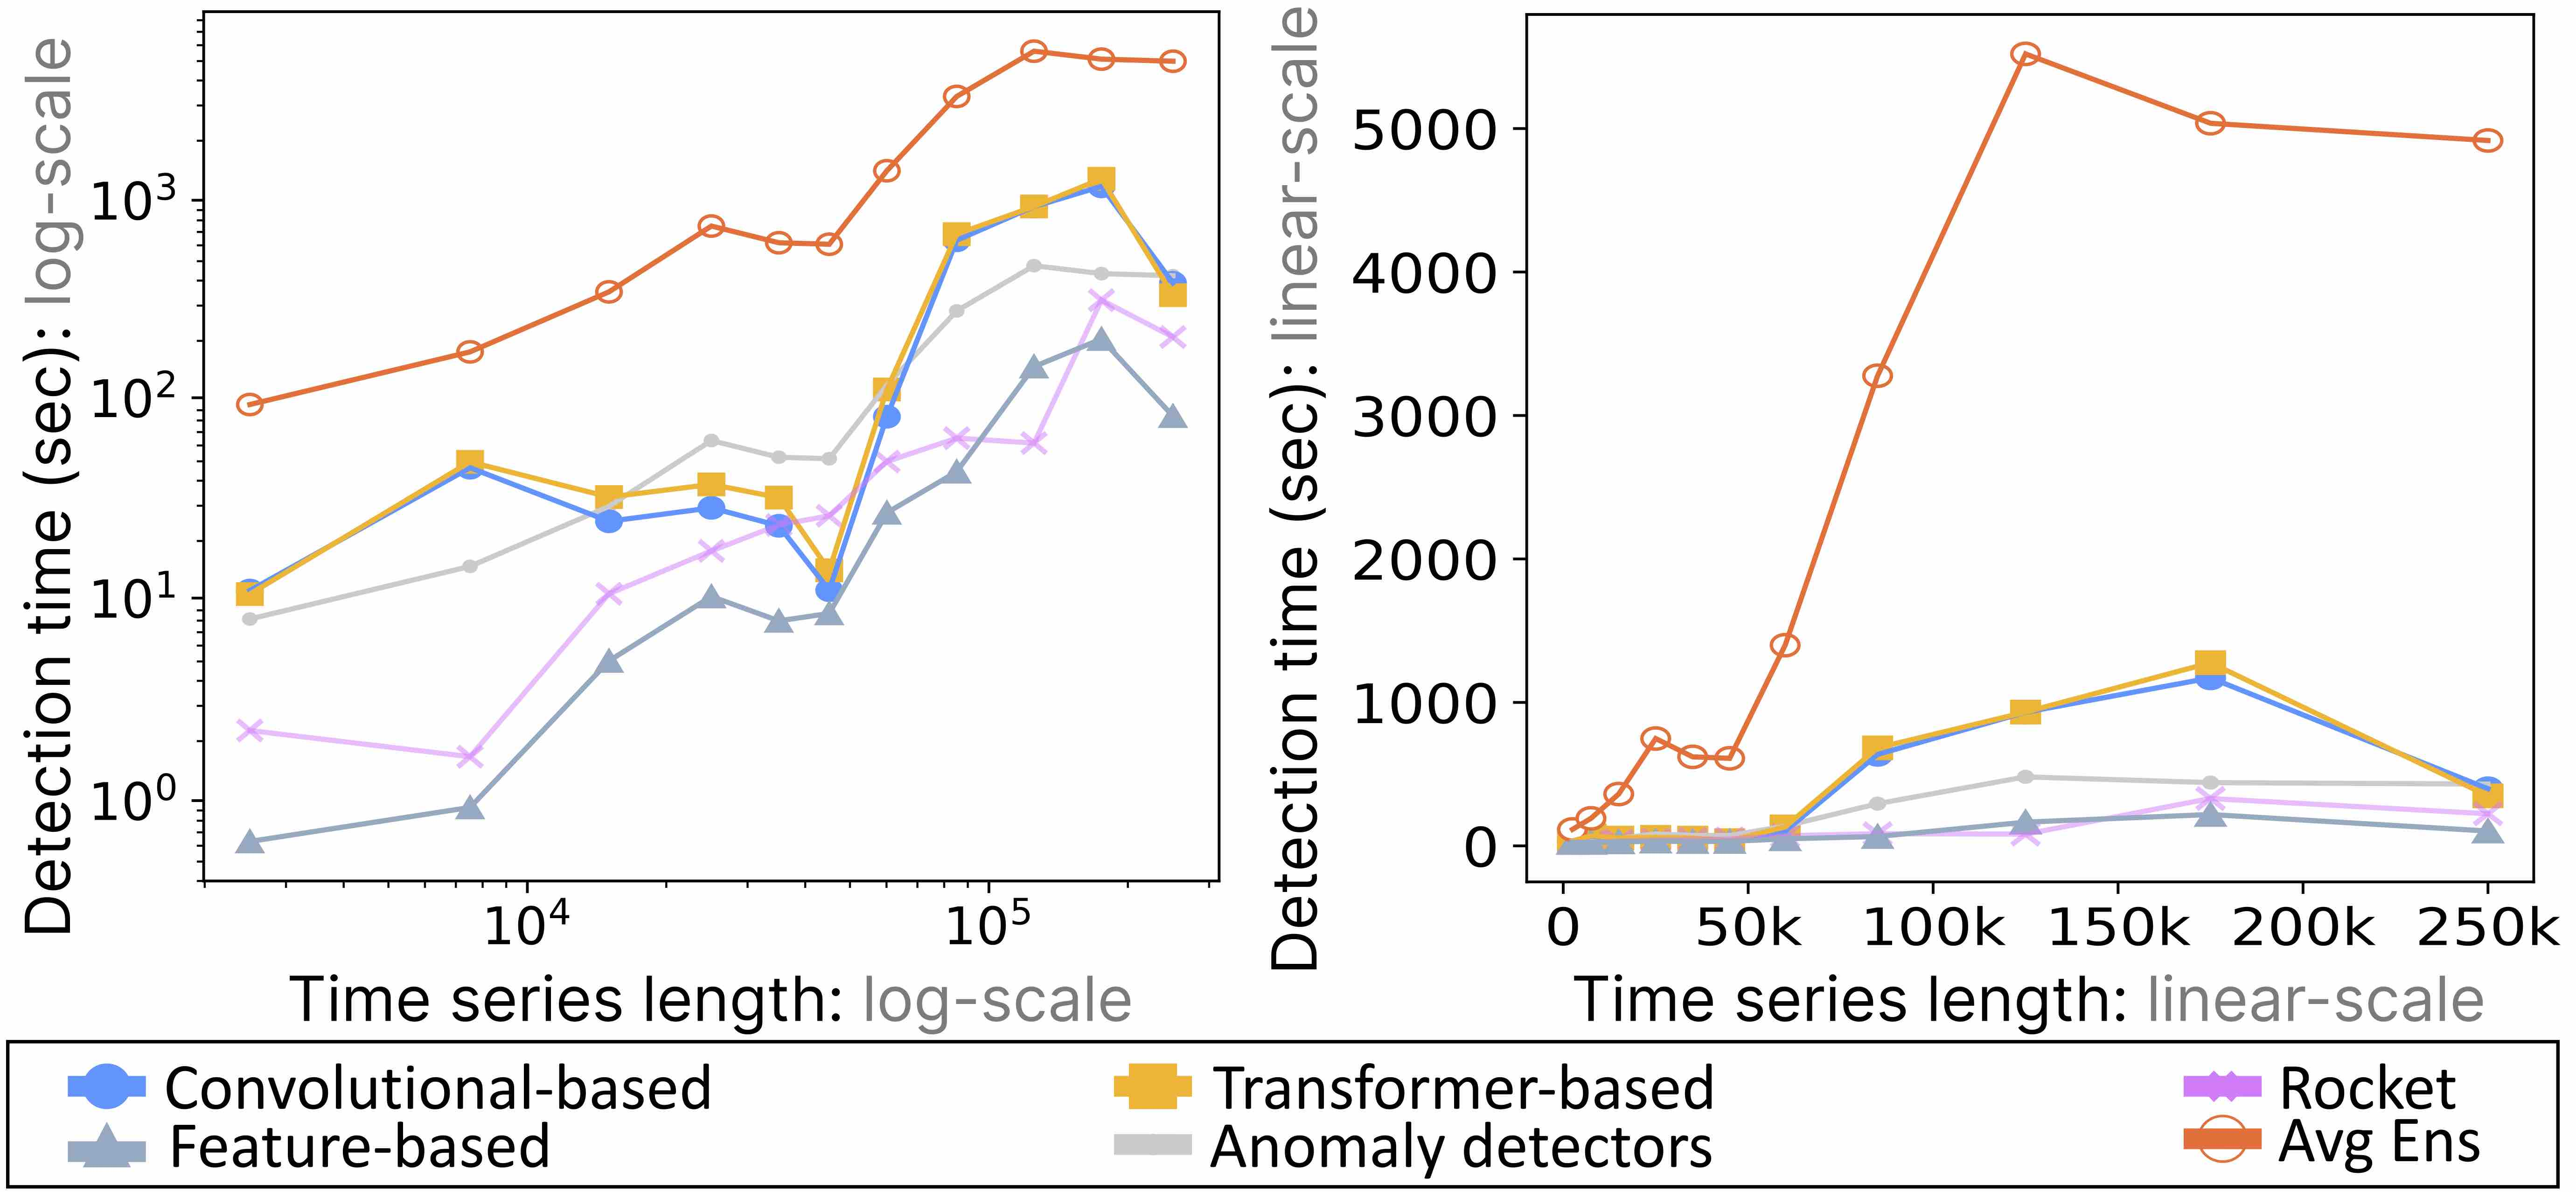
\includegraphics[width=\linewidth]{figures/Fig7.jpg}
        \caption{Execution time vs. length of model selection methods.}%for time series in TSB-UAD.}
        \label{fig:scalability}
\end{figure}

\subsubsection{\textbf{Model selected distribution}}
\label{exp:distribution}

We then inspect the prediction and the detector chosen by the model selection approaches. In this section, we consider only $resnet$-$1024$, $convnet$-$128$, $sit$-$stem$-$512$, $rocket$-$128$, and $knn$-$1024$. These approaches are the best models (using either AUC-PR or VUS-PR) based on the analysis conducted in Section~\ref{exp:overalleval} (you may find additional information on AUC-PR evaluation in our website~\cite{ourwebsite}).

Figure~\ref{fig:classif_distrib} (a) depicts the distribution of the chosen detectors by the 5 model selection approaches mentioned above for the entire TSB-UAD benchmark. The black bar corresponds to the true labels (i.e., the best detectors). We observe from Figure~\ref{fig:classif_distrib} (a) that $rocket$-$128$ and $knn$-$1024$ are significantly overestimating the detector NormA (as well as LOF for $rocket$-$128$ and HBOS for $knn$-$1024$), whereas $resnet$-$1024$, $convnet$-$128$, and $sit$-$stem$-$512$ are matching the correct distribution of detectors (we observe a slight underestimation of LOF, IFOREST1 and an overestimation for POLY).

Moreover, we measure the prediction distribution differences for time series containing sequence anomalies (Figure~\ref{fig:classif_distrib} (b.1)) and point anomalies (Figure~\ref{fig:classif_distrib} (b.2)), and for time series containing only one anomaly (Figure~\ref{fig:classif_distrib} (c.1)) and multiple anomalies (Figure~\ref{fig:classif_distrib} (c.1)). We first observe that predictions of model selection methods are significantly different for time series with sequence and point anomalies. More specifically, $resnet$-$1024$, $convnet$-$128$, and $sit$-$stem$-$512$ are correctly selecting the method CNN, whereas $rocket$-$128$ and $knn$-$1024$ are over selecting LOF and NormA for time series containing point anomalies. However, for sequence anomaly, as it represents most of the TSB-UAD benchmark, the prediction distribution is similar to the one over the entire benchmark. Moreover, the correct predictions of $resnet$-$1024$, $convnet$-$128$, and $sit$-$stem$-$512$ for time series containing point anomalies are interesting, as this information is not provided in the training step. Therefore, these models found discriminant features in the time series that indicate whether it might contain a point or a sequence anomaly.

We, finally, measure the differences between the prediction distribution of model selection methods between time series containing unique and multiple anomalies. The true labels (black bars in Figure~\ref{fig:classif_distrib} (c.1) and (c.2)) indicate that, for unique anomalies, the best detectors are LOF, NormA, and HBOS and for multiple anomalies, the best detector is NormA. We observe that all model selection approaches correctly select LOF, NormA, and HBOS for time series containing a unique anomaly. The latter indicates that model selection methods can extract discriminant features that indicate if one time series is more likely to have multiple anomalies.


\subsubsection{\textbf{Execution Time Evaluation}}

We now discuss the execution time of model selection methods. In this section, we focus only on the detection time (i.e., the number of seconds required by a method to predict the detector to use and to run it). Figure~\ref{fig:overall_res} (b) depicts the detection time (in log scale) for each method and detector in the TSB-UAD benchmark. We first observe that the Avg Ensemble required to run all detectors is significantly slower than the rest. Then, all model selection methods are of the same order of magnitude as the detectors. We also observe that all the deep learning methods are slower than the feature-based approaches. This is surprising because the detection time mainly depends on the chosen detector. Overall, we conclude that method selection is the only viable solution that outperforms the existing anomaly detection methods and can be executed in the same order of magnitude of time. Finally, we depict in Figure~\ref{fig:scalability} the scalability of model selection methods versus individual detectors and the Avg Ensemble approach when the time series length increases. We observe that, on average, the execution time of model selection approaches increases similarly to the execution time of individual detectors when the time series length increases. We also observe that the time series length significantly impacts the Avg Ensemble approach execution time. The latter shows the scalability issue of the Avg Ensemble approach for very large time series.

\begin{figure}
    \centering
    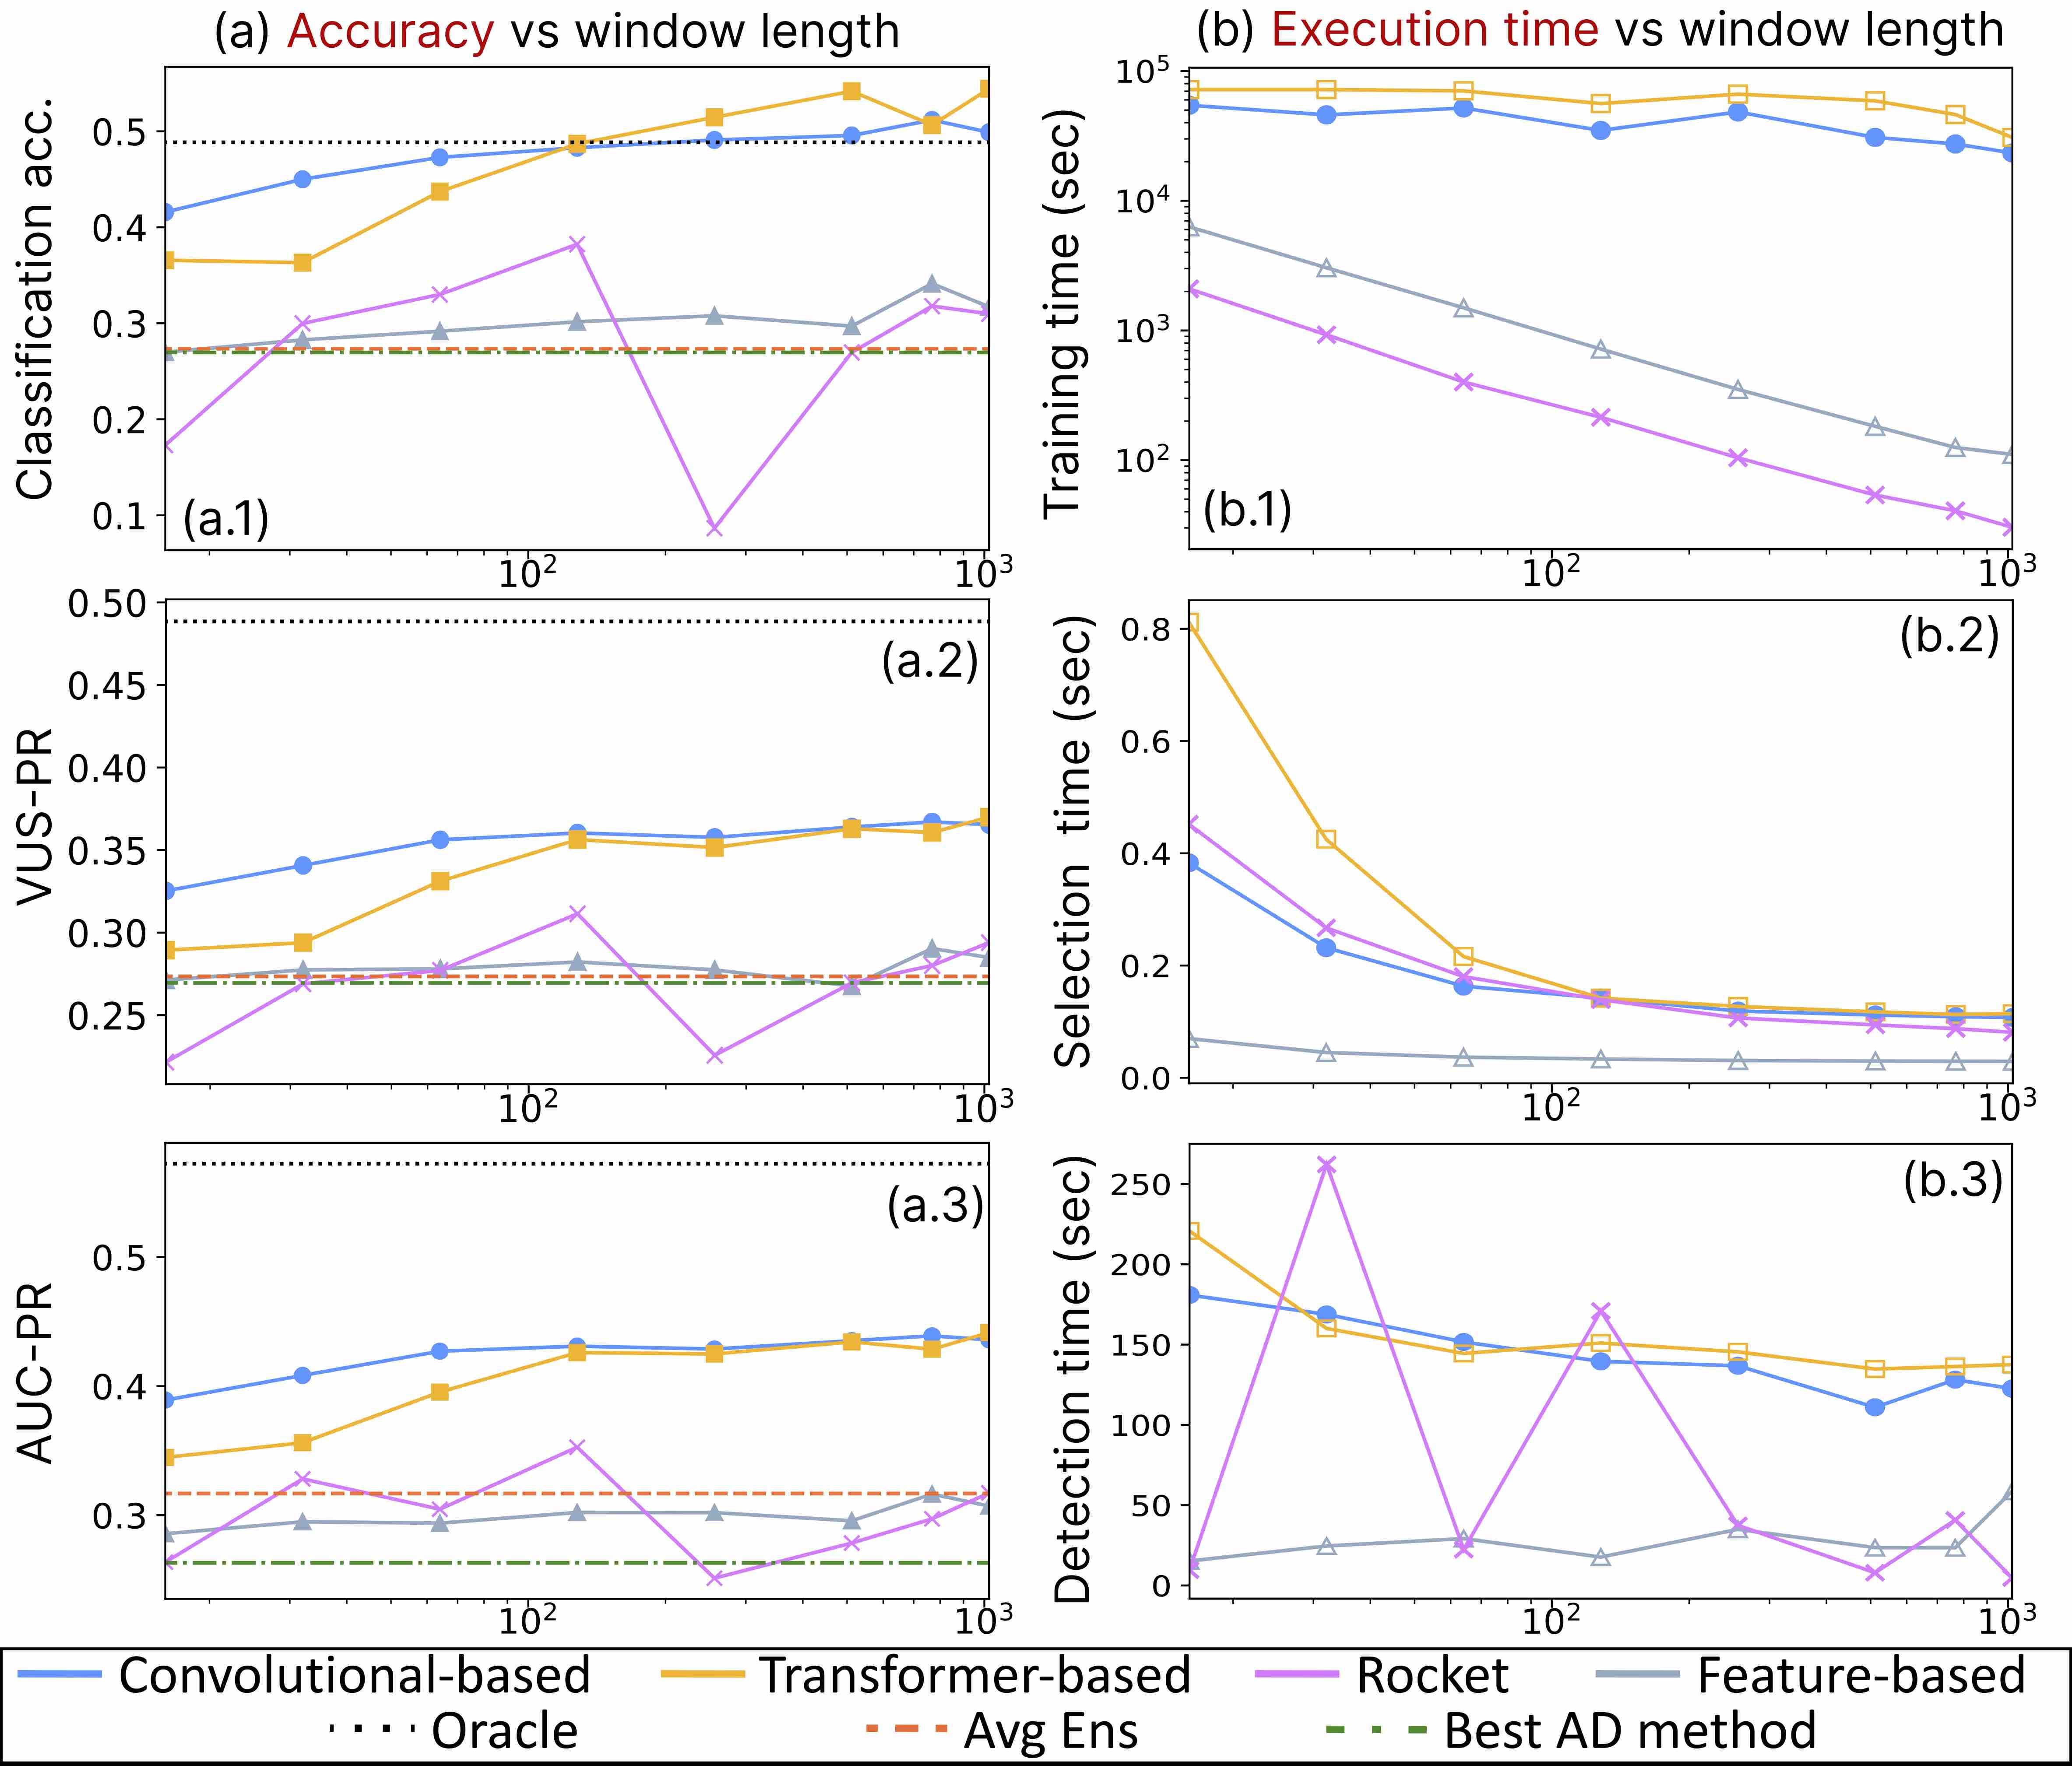
\includegraphics[width=\linewidth]{figures/Fig8.jpg}
        \caption{(a) Accuracy ((a.1) classification accuracy, (a.2) VUS-PR and (a.3) AUC-PR) and (b) execution time ((b.1) training time, (b.2) selection time and (b.3) detection time) versus window length $\ell$.}
        \label{fig:lengthinfl}
\end{figure}

\subsection{Influence of the Window Length}
\label{exp:windowlength}


In this section, we analyze the influence of the window length on classification accuracy (Figure~\ref{fig:lengthinfl} (a.1)), anomaly detection accuracy (Figure~\ref{fig:lengthinfl} (a.2) and (a.3)) and execution time (Figure~\ref{fig:lengthinfl} (b)). We perform the analysis per group of methods (i.e., average for Convolutional, Transformer, \journalv{Rocket}, and Feature-based methods).

We first observe in Figure~\ref{fig:lengthinfl} (a) that Convolutional-based and Transformer-based methods outperform the best anomaly detection methods (green dashed line in Figure~\ref{fig:lengthinfl} (a.2) and (a.3)), the Avg Ensemble approach (orange dotted line in Figure~\ref{fig:lengthinfl} (a.2) and (a.3)), Rocket and Feature-based methods, whatever the length used with regard to the classification accuracy, VUS-PR, and AUC-PR. We also observe that Transformer-based approaches are less accurate for shorter lengths (less than 100 points), whereas the accuracy of Convolutional-based approaches is stable regardless of the window length. Overall, Transformer and Convolutional-based approaches converge to the same anomaly detection accuracy (both for VUS-PR and AUC-PR) when the window length increases.

\begin{figure}
    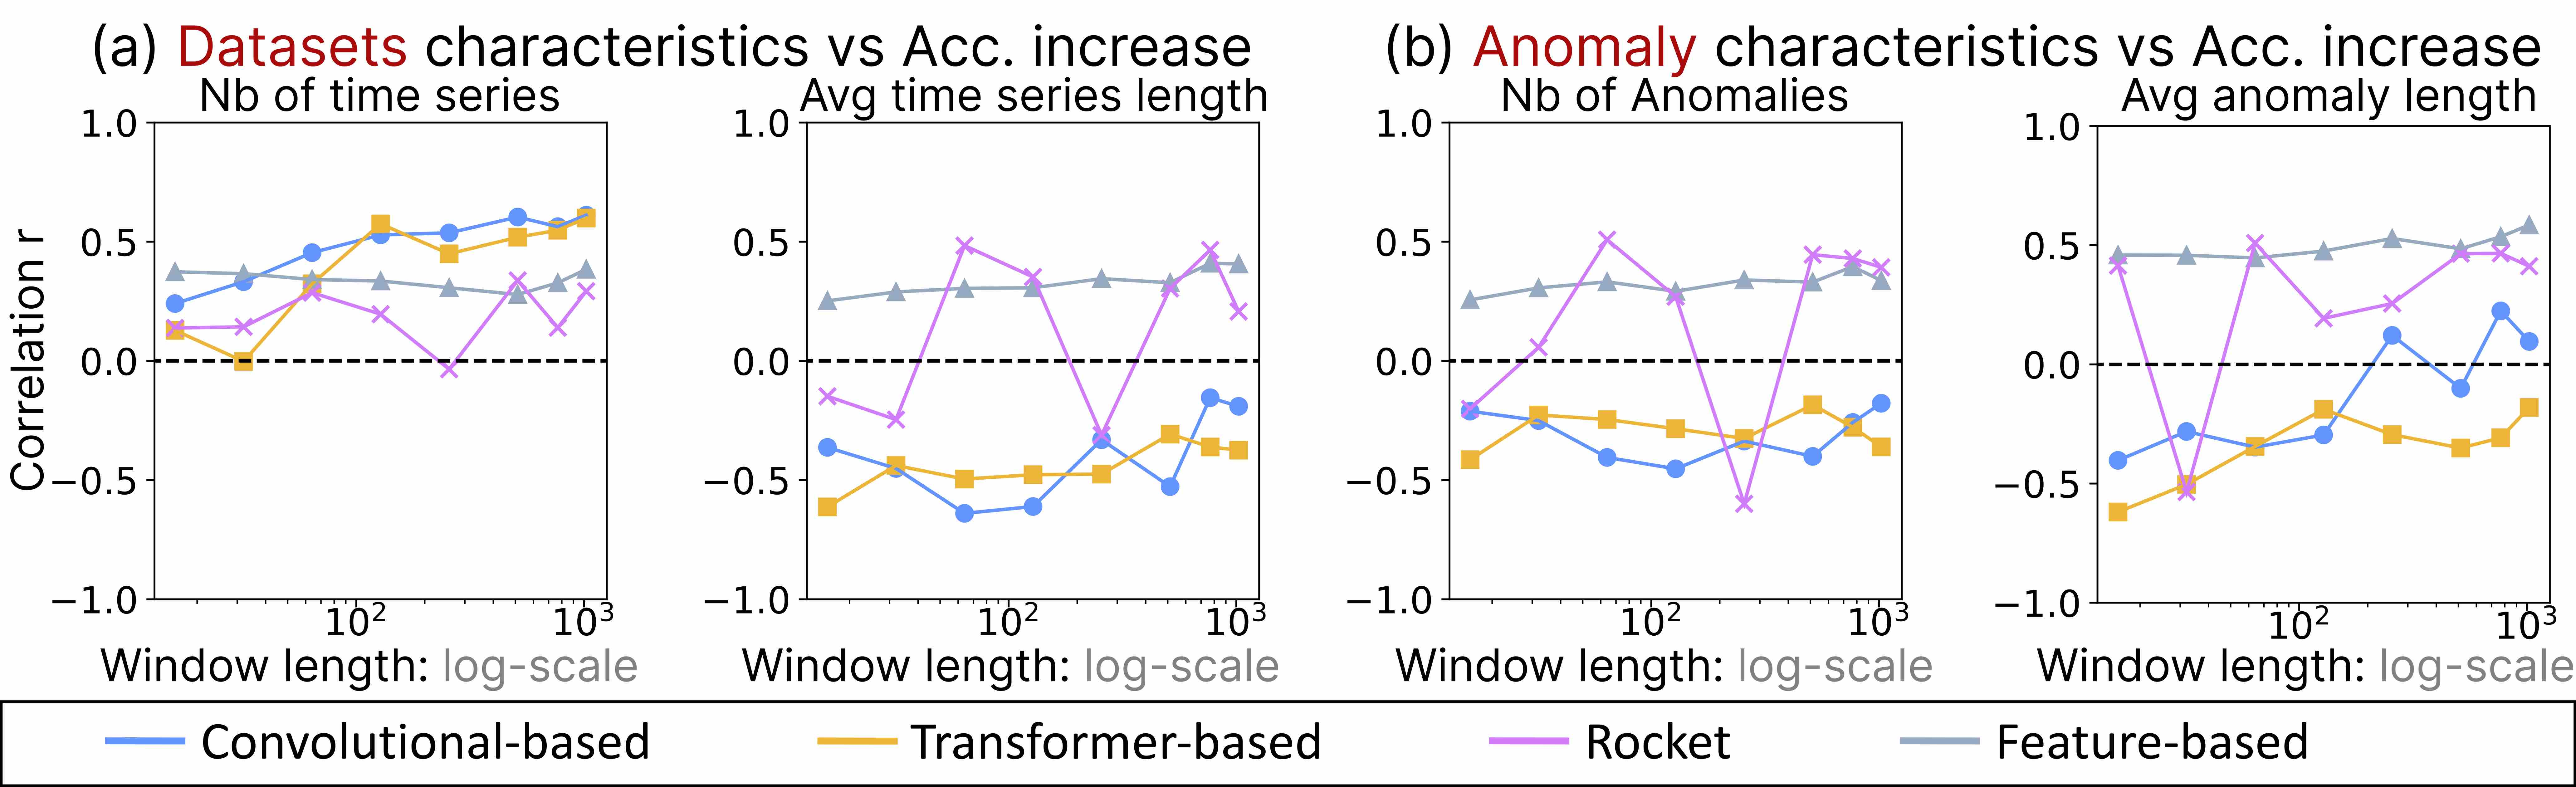
\includegraphics[width=\linewidth]{figures/Fig9.jpg}
    \caption{Correlation between accuracy and time series characteristics vs. the window length used to train the model selection methods.}
    \label{fig:infl_charac}
\end{figure}

Furthermore, we observe that both \journalv{Rocket} and Feature-based approaches are significantly faster to be trained than Convolutional and Transformer-based approaches (Figure~\ref{fig:lengthinfl} (b.1)). We make the same observation for selection time  ((Figure~\ref{fig:lengthinfl} (b.2))). For the detection time, we observe that \journalv{Rocket} execution time is very unstable when compared to the other approaches. The latter means that the choice of length strongly impacts the model selection performed by \journalv{Rocket}, leading to very diverse selection and execution times.

In the general case, we can make the following two statements: (i) \journalv{A large window length results in faster selection time for the model selection process and better accuracy for Convolutional and Transformer-based approaches.} (ii) Feature-based approaches are significantly faster but less accurate than Convolutional-based and Transformer based approaches, \journalv{regardless of} the window length used.


\subsection{Influence of Datasets and Anomaly Types}
\label{exp:datasets}

In this section, we evaluate the influence of datasets and anomaly characteristics on model selection accuracy. We perform the analysis per group of methods (i.e., average performances for Convolutional, Transformer, Rocket, and Feature-based methods).

For this experiment, we evaluate the dataset and anomaly characteristics (i.e., the number of time series, the average length of the time series, the average number of anomalies and the average anomaly length). Figure~\ref{fig:infl_charac} depicts these characteristics (x-axis) versus the average increase of accuracy (VUS-PR of the model selection method subtracted by VUS-PR of the best anomaly detection method for each dataset) for each model selection method using a given window length. For instance, if a point (one model selection method on one dataset) is positive (above the black dotted line), then this model is more accurate on the corresponding dataset than the best anomaly detection method selected on this same dataset. %Figure~\ref{fig:infl_charac} (1) shows a specific example for window length $\ell=1024$. Figure~\ref{fig:infl_charac} (2) shows the correlation values (trend of the different lines in Figure~\ref{fig:infl_charac} (1)) versus the window length.
We generally observe low correlations between dataset and anomaly characteristics (i.e., $-0.6<r<0.6$). With such correlation values, we cannot conclude any factual statement on the impact of these characteristics and the model selection methods' performances. However, we can make the following observations.

%First, Figure~\ref{fig:intro_fig} (a.1) shows that all model selection methods (with a window length $\ell=1024$) are more likely to be accurate on large datasets. 
First, Figure~\ref{fig:infl_charac} (a) shows that the number of time series is impacting more substantially Convolutional and Transformer-based approaches with large window lengths. For the average time series length, only Feature-based approaches are positively impacted. On the contrary, Convolutional and Transformer-based approaches are less accurate when the average time series length is increasing. These observations imply that Convolutional and Transformer-based are more affected by the number of examples in the dataset rather than the length of each instance. In contrast, Feature-based approaches benefit from both more and large instances.

Then, Figure~\ref{fig:infl_charac} (b) shows that Feature-based approach accuracy is increasing with the anomaly characteristics, whereas these characteristics either do not or negatively impact Convolutional and Transformer-based methods. More specifically, we observe that Feature-based approaches (regardless of the window length) are more accurate with time series containing large anomalies, and Convolutional-based approaches are less accurate (irrespective of the window length) when the number of anomalies increases.

We note that Rocket's correlation with the dataset and the anomaly characteristics is unstable. The latter is explained by the fact that the model prediction of Rocket is very sensitive to the window length (as described in Section~\ref{exp:windowlength}). Thus, it is impossible to make a conclusion on Rocket's performances, datasets, and anomalies.


\subsection{Detection vs Classification Accuracy}
\label{exp:detectionvsclass}

In this section, we analyze the relationship between the model selection methods' classification accuracy and the resulting anomaly detection accuracy. In this experiment, we consider VUS-PR as anomaly detection measures. For this experiment, we extend the definition of $Oracle$ (introduced in Section~\ref{sec:problem_def}) as follows:

\begin{definition}
    We define $Oracle_{k,j}$ as a hypothetical model selection method that has a classification accuracy of $k \in [0,1]$ and selects the $j^{th}$ best detector (among $m$ detectors) in cases of misclassification. Thus, $Oracle_{1,1}$ always selects the best detector, and $Oracle_{0,m}$ always selects the worst detector. Finally, we define $Oracle_{k,R}$ as the model selection method with a classification accuracy of $k \in [0,1]$ and that randomly selects a detector in misclassification cases.
    \end{definition}

\begin{figure}
    \centering
    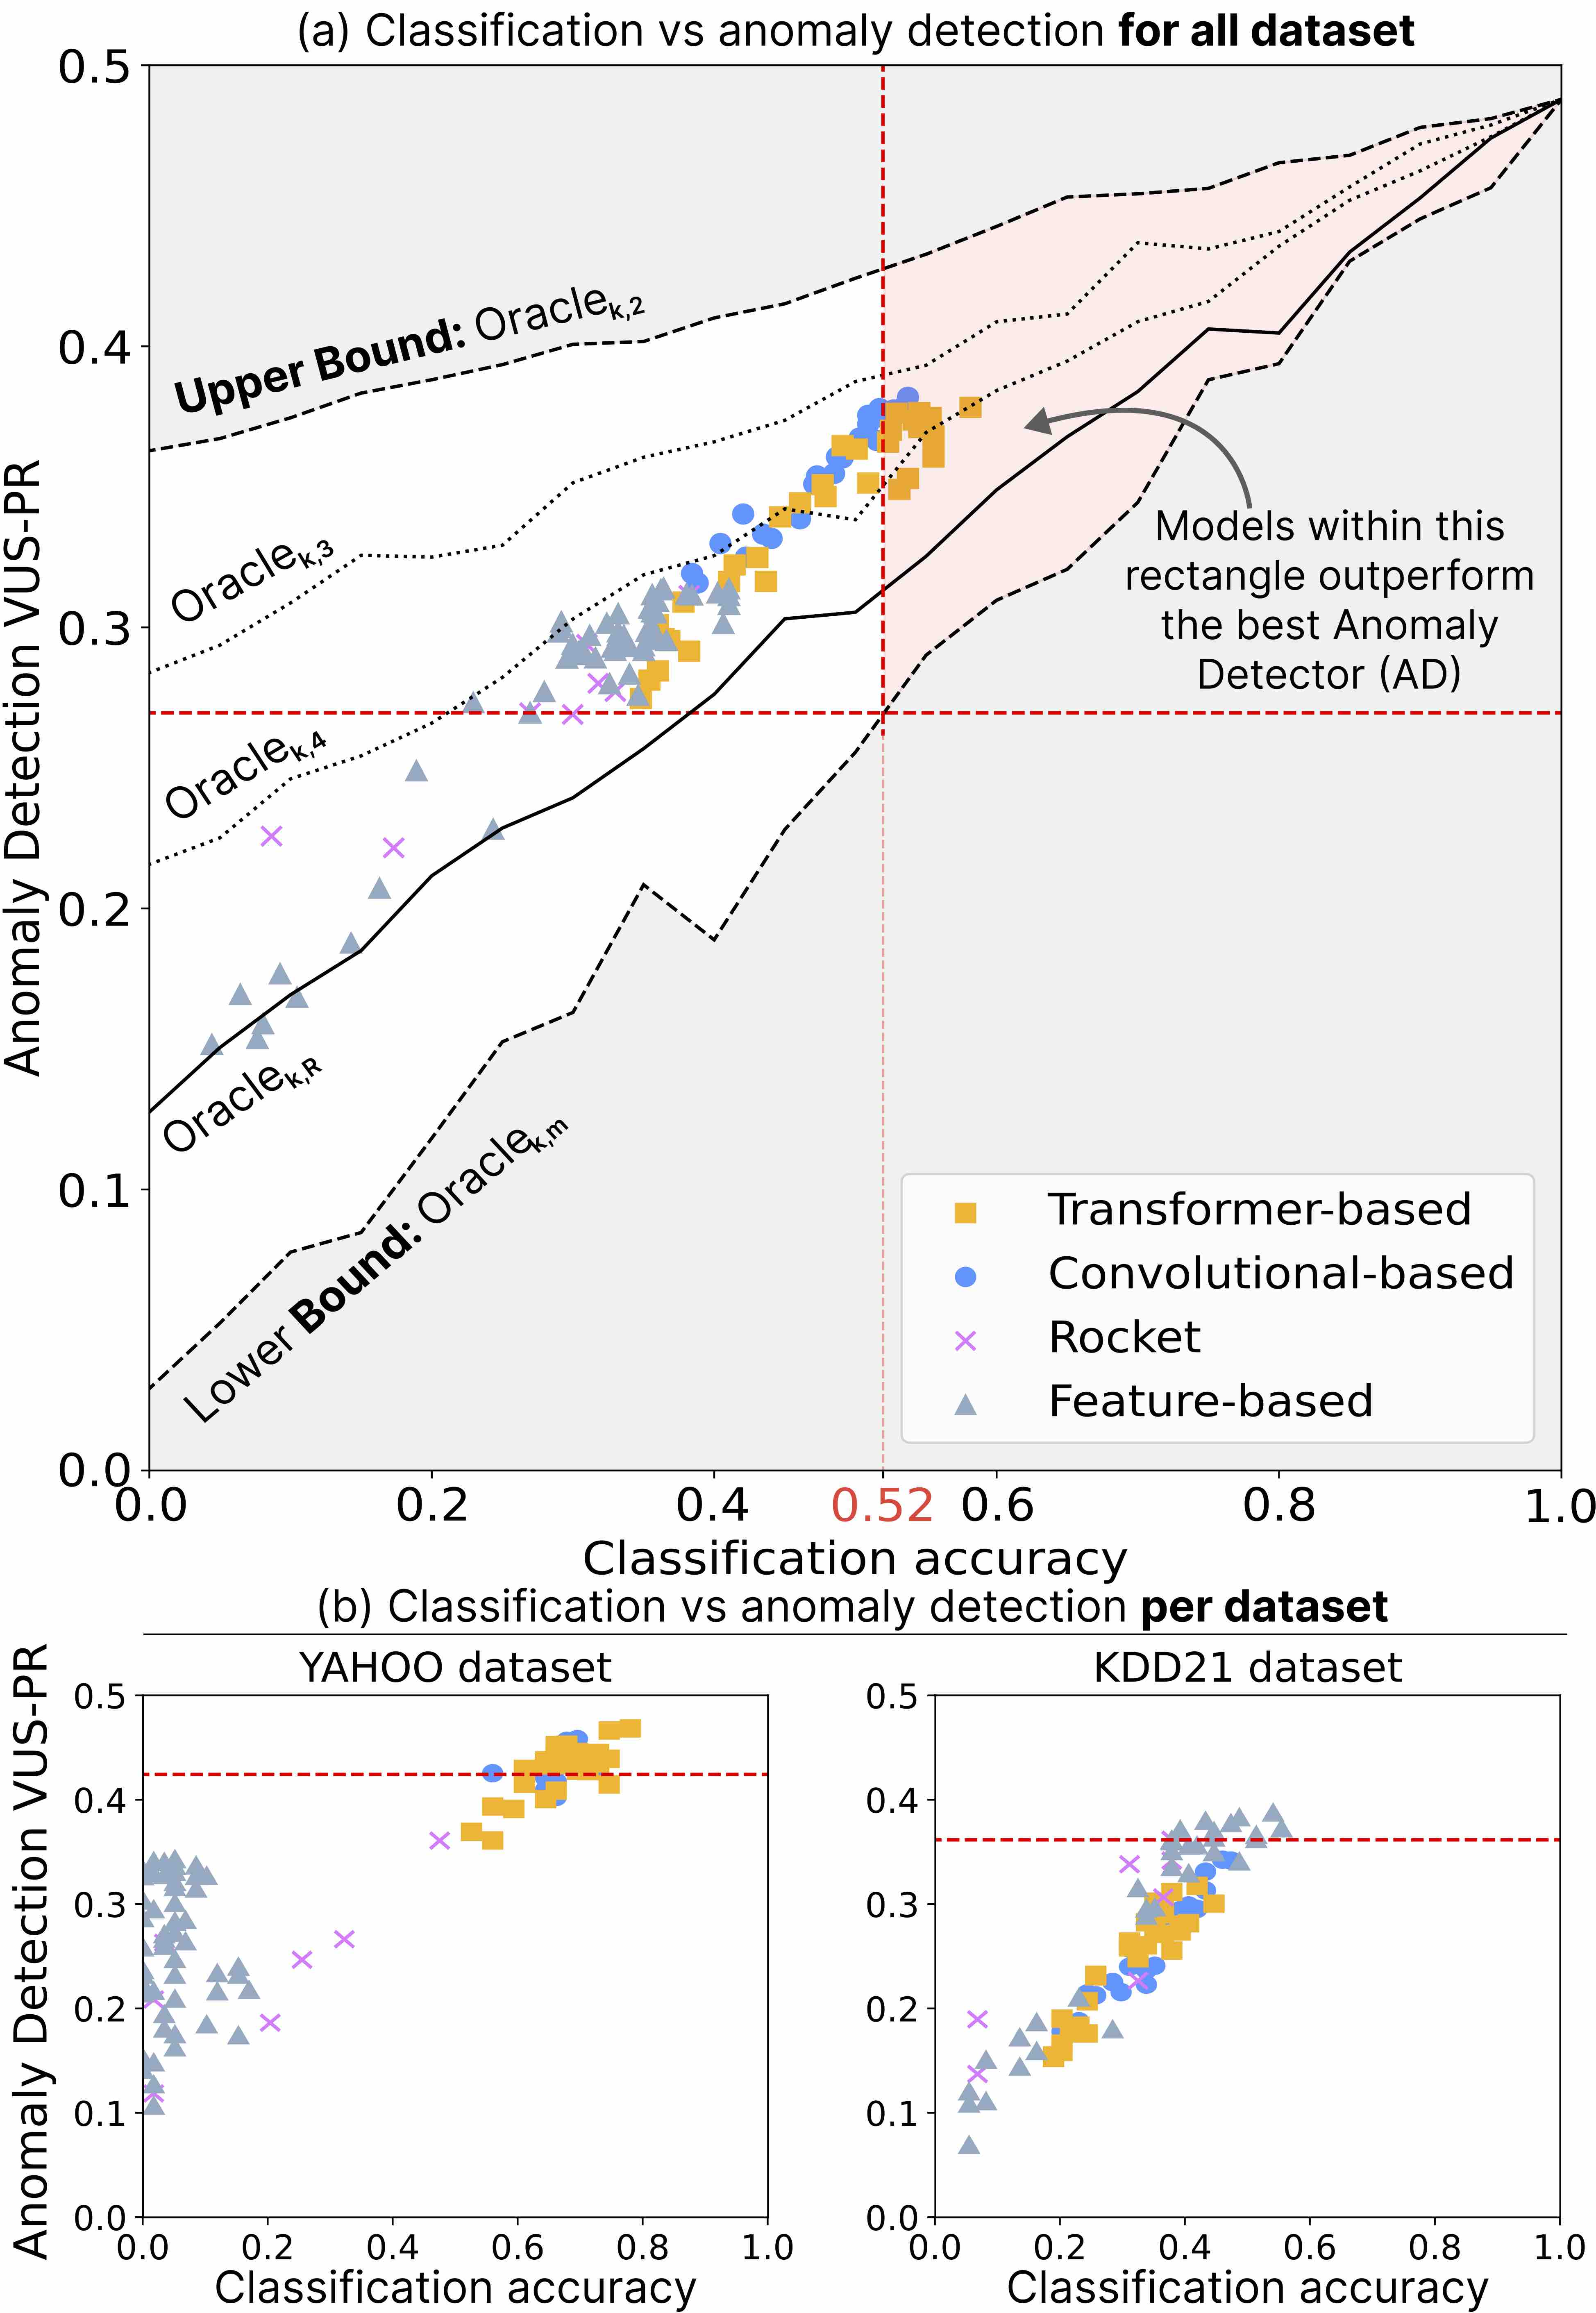
\includegraphics[width=\linewidth]{figures/Fig10.jpg}
        \caption{Classification accuracy versus anomaly detection accuracy (VUS-PR) for (a) all datasets and (b) two specific datasets.}
        \label{fig:class_AD}
\end{figure}


\begin{figure*}
    \centering
    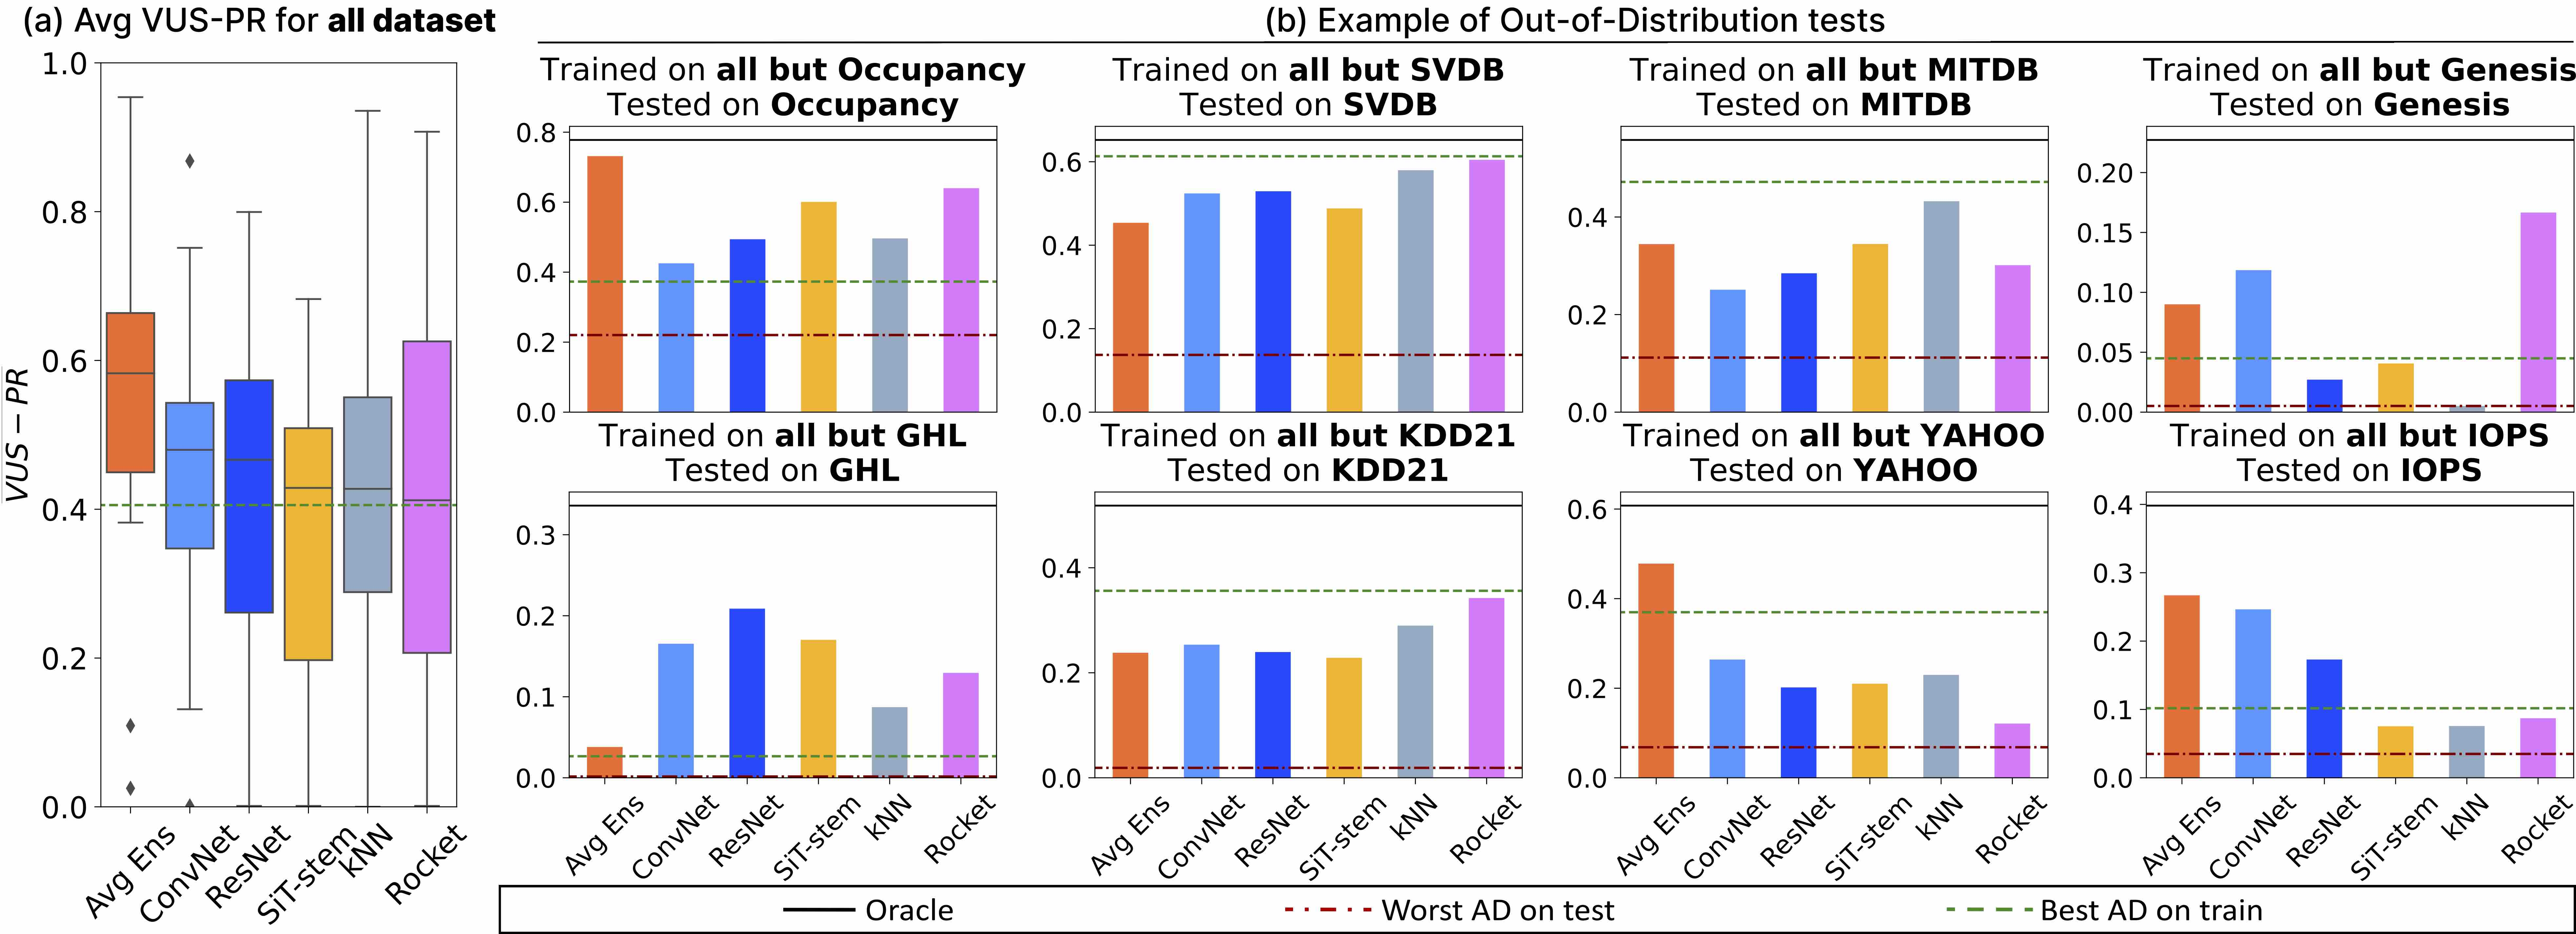
\includegraphics[width=\linewidth]{figures/Fig11.jpg}
        \caption{Out-of-distribution experiment, when model selection algorithms are trained on all but one dataset. (a) results for each dataset (when not included in the training set) and (b) average results.
    }
        \label{fig:one_vs_all}
\end{figure*}

Figure~\ref{fig:class_AD} depicts the latter comparison for all datasets (Figure~\ref{fig:class_AD} (a)), and two specific datasets (Figure~\ref{fig:class_AD} (b)). We first observe a strong correlation between classification accuracy and anomaly detection accuracy for each specific dataset and, on average, all datasets. However, methods belonging to different families (e.g., Feature-based or Transformer-based) are not performing the same. For instance, Figure~\ref{fig:class_AD} (a) shows that Feature-based approaches are not accurate for YAHOO but are the best models for KDD21. Overall, we observe that Convolutional and Transformer-based are more accurate in classification and anomaly detection (Figure~\ref{fig:class_AD}(b)). 

We also depict in Figure~\ref{fig:class_AD} (a) the lines corresponding to $Oracle_{k,2}$, $Oracle_{k,3}$, $Oracle_{k,4}$, $Oracle_{k,R}$, and $Oracle_{k,m}$. For a given classification accuracy, $k$, $Oracle_{k,2}$, and $Oracle_{k,m}$ correspond to the upper and lower bounds. The latter means that model selection approaches with a given classification accuracy will be within the previously mentioned upper and lower bounds for VUS-PR (i.e., in the grey zone in Figure~\ref{fig:class_AD} (a)). Thus, any model selection method that has a classification accuracy above 0.53 (intersection between the two dashed red lines) is better than the current best anomaly detection method in TSB-UAD (i.e., red dashed line in Figure~\ref{fig:class_AD} (b)). 
This is true only for a few Convolutional- and Transformer-based methods in our experiments.

Moreover, we compare the positions of the model selection methods with regard the $Oracle_{k,3}$, $Oracle_{k,4}$, and $Oracle_{k,R}$. We observe in Figure~\ref{fig:class_AD} (b) that almost all methods are above $Oracle_{k,R}$. The latter means that the model selection methods do not randomly select detectors when the wrong detector is selected. Moreover, most models follow the $Oracle_{k,4}$ line. The latter indicates that the models averagely select the third-best in case of misclassification. Finally, the observations discussed above demonstrate three important statements: (i) classification accuracy can be used as a proxy for anomaly detection accuracy, and without computing the anomaly detection accuracy, we can provide an anomaly detection accuracy lower and upper bounds; (ii) the gap between the best model selection and the top right corner of the grey zone shows that there is a significant margin for improvement for future work; (iii) the vertical gap between the models and the upper bound ($Oracle_{k,2}$) shows that there is an important margin of improvement in the prediction rank: a model with the same classification accuracy can gain up to $0.1$ VUS-PR if it better selects models.


\subsection{Out-of-Distribution Experiments}
\label{exp:sup2unsup}

At this point, we tested the performances of the model selection methods when trained on a subset of the benchmark with examples from all 16 datasets available. \journalv{These results are interesting when we suppose that a user wants to analyze datasets similar to the one considered in the benchmark.} In some cases, though, we may want to analyze time series that are not similar to any of those in the benchmark. Therefore, in this section, we measure the ability of the model selection methods to be used in an unsupervised manner (i.e., used for datasets that are not similar to the one used in the training set). We run the following experiment. We train the model selection methods on 15 datasets (70\% of the time series for training and the other 30\% for validation), and we test on the remaining one. We try all 16 possible test partitions, and (for brevity) report 8 of these tests in Figure~\ref{fig:one_vs_all} (a). We only show the results for the best-performing model selection methods listed in Section~\ref{exp:distribution}\journalv{, namely, $resnet$-$1024$, $convnet$-$128$, $sit$-$stem$-$512$, $rocket$-$128$, $knn$-$1024$ and the Averaging ensemble for comparison. For simplicity, we only report the model's name without the window length.}

Figure~\ref{fig:one_vs_all} (a) \journalv{illustrates} the normalized VUS-PR (\journalv{denoted} $\overline{VUS\text{-}PR}$) for all 16 tests: \journalv{$\overline{VUS\text{-}PR}$} of 1 corresponds to the VUS-PR of the \emph{Oracle} on each test, while 0 corresponds to the worst anomaly detection methods on each test. This figure shows that, in the unsupervised case, the Avg Ensemble outperforms all model selection methods, as well as the best anomaly detection method based on the accuracy performance measured on the train set (dotted green line in Figure~\ref{fig:one_vs_all} (a)). The latter means that, for unknown datasets, it is safer to run all existing anomaly detection methods and average their scores. Knowing that such ensembling methods are not scalable (as shown in Figure~\ref{fig:overall_res}), Figure~\ref{fig:one_vs_all} (a) shows that ConvNet or ResNet is still a better choice than choosing the best anomaly detection method selected on train data (i.e., known data). However, kNN, Rocket, and SiT-stem are only slightly more accurate than the best anomaly detection method.

Figure~\ref{fig:one_vs_all} (b) depicts the average accuracy for 8 out of the 16 tests \journalv{(datasets excluded from the training set and used for testing)}. We observe very different results. First, for Electrocardiograms (SVDB), \journalv{neither} the model selection methods \journalv{nor} the Avg. Ensemble outperform the best anomaly detection method (selected on the training set). \journalv{However, for various kinds of sensor data (GHL and Occuopancy), model selection methods and the Avg Ensemble do outperform the best anomaly detection method (again selected on the training set).}  \journalv{This difference} can be explained by the fact that ECGs exhibit less \journalv{diverse} behaviors (i.e., repetitive normal patterns and similar anomalies) than other sensor data. \journalv{Consequently,} it is more likely to have one method in the benchmark that performs well on all \journalv{ECG} time series. \journalv{This observation is supported by the fact that the performance of the best anomaly detection method closely matches that of the Oracle for SVDB.}

These observations lead to the following remarks: (i) there is a significant margin of improvement when using the existing time series classifiers as model selection methods in the unsupervised case; (ii) when a new dataset arrives, it is safer in the general case to use an ensembling method such as the simple average of all anomaly scores; and (iii) for heterogeneous datasets (without known and repetitive normal or abnormal patterns), classifiers as model selection (mainly convolutional-based classifiers) can be used even though similar time series are not in the training set.